\documentclass{article}
\usepackage{graphicx}
\usepackage{amsmath} 
\usepackage{fixltx2e}
\usepackage{hyperref}
\RequirePackage{titlesec}
\begin{document}
	\begin{center}
		\LARGE  {\textbf{SHIVANI JINDAL}}
	\end{center}
	\noindent
	\begin{figure}
		\begin{center}
			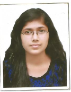
\includegraphics{Capture.PNG}
		\end{center}
	\end{figure}

	\noindent\makebox[\linewidth]{\rule{\paperwidth}{0.4pt}}


	\textbf{\underline{Address:}}
	\hfill
	\textbf{\underline{contact:}}\\
		Wz- 528C/1 Sri Nagar, Rani Bagh, 
	\hfill
		9717288483
		\\New Delhi-110034
	\hfill
		jindalshivani11@gmail.com
	\section{Career Objective}
		My main objective is to be an Android App developer by making apps that will benefit common people to maintain a healthy living. I am a quick learner and appreciate new things in life. I am also interested in Machine learning with artifical intelligence and would want to pursue this forward in order to make my Android part very strong.
	\section{Education And Academic Qualification}
		\begin{tabular}{||l | l | l | l | l||}
			\hline
			Deg/Sem & Institute & University/Board & Passing Year & Percentage/CGPA\\
			\hline
			Semester 2 & B.V.C.O.E & G.G.S.I.P.U & 2018 & 8.67 \\
			\hline
			Semester 1 & B.V.C.O.E & G.G.S.I.P.U & 2018 & 8.963\\
			\hline
			12$^{th}$ Board & KIIT WORLD SCHOOL & CBSE & 2016 & 83.4\%\\
			\hline
			10$^{th}$ Board & V.B.P.S & CBSE & 2014 & 9.2\\
			\hline
		\end{tabular}

	\section{Projects}
		\begin{enumerate}
			\item \href{https://github.com/jindalshiva/heart}{ Health issues are becoming common nowadys; probably due to new advanced lifestyle. An android app developed by me that would help users in improving health issues which is very easy to use just by providing details of height, weight and age. Afterwards as per these parameters app will provide them with a health chart that they would follow. There is also a label detector to calculate total amount of calories that any food item contains. Moreover, it also contains a blood pressure detector system.}
			\item \href{https://github.com/jindalshiva/GooglePlacesGoogleMaps} { Google map app: This app is very similar to google maps; I made this app to learn how to use google maps in android studio. It contains one search view wherein if you provide it with any location It will take you to the location. To build this app i used google maps api and google places api.}
			\item \href{https://github.com/jindalshiva/ISTY_1.2.3-master-master} { Home automation: this was a big initiative taken by ISTE society of my college where many things included like web development, IOT, android Development. I participated and made this android app. This app is connected to firebase. First user need to login to app then it will direct them to a page where he needs to add devices and when he clicks on the 'ON' button then light will be switched on. User can also put a timer.}

		\end{enumerate}
	\section{Training And Internship}
		\begin{itemize}
			\item {Completed summer internship with Marconi Society(Celestini) in collaboration with IIT-Delhi.}
			\item {Attended workshop on Internet Of Things organized by CETPA INFOTECH PVT LTD.}
			\item \href{https://classroom.udacity.com/courses/ud836}{Udacity course: This course was very helpful this was my second course here i learn various things like user input how can we control user interface with user input and how can we create one good app.}{AUDITED}
			\item \href{https://classroom.udacity.com/courses/ud839}{udacity course: This course takes me to next level in android studio where i come to know about intents how can i have multiscreens in my app how can i go from one activity to another activity. }{AUDITED}
			\item \href{https://classroom.udacity.com/courses/ud834}{Udacity course: This was a very basic course that will help you to learn the basics of user interface means xml.}{AUDITED}
		\end{itemize}
	\section{Research And Publications}
		\begin{enumerate}
			\item {NULL}
		\end{enumerate}
	\section{Technical Skills}
		\begin{itemize}
			\item {Programming Languages: C,C++}
			\item {Markup languages: HTML,CSS}
			\item {Query language: SQL}
			\item {Graphics: Photoshop, Blender}
			\item {Technical Skills: Android Apps Development}
			\item {Works on APIs}
			\item {Operating Systems works upon: windows, mac osx, Ubuntu, android}
		\end{itemize}
	\section{Soft Skills}
		\begin{enumerate}
			\item {LeaderShip Skills}
			\item {Team Work}
			\item {Flexibility}
		\end{enumerate}
	\section{Extracurricular Activities}
		\begin{itemize}
			\item { First in essay writing competition by district election office }
			\item { Second in Patriotic group song}
			\item { Consolation in folk group song}
			\item { Volunterring at NSS B.V.C.O.E}
		\end{itemize}
	\section{Co- Curricular Activities}
		\begin{enumerate}
			\item {I am android mentor in societies- ACM, DSC-WTM}
			\item{ Got the third position in \textbf{mind the app} a 6 hr competition that was held in \textbf{I.G.D.T.U.W }}
			\item {Got second position in \textbf{HACK@BVP 2.O} a 24 hr hackathon that was organised by \textbf{B.V.C.O.E}}
			\item { Participated in \textbf{Paytm - Build for India Hackathon} held in \textbf{IIT- DELHI}}
			\item { Won \textbf{Eyantra-- the biggest robotics competition} held in \textbf{IIT - BOMBAY}}
		\end{enumerate}
	\section{Personal Details}
		\begin{tabular}{ll}\\
			\textsc{Father's Name: }& Nand Kishor Jindal\\
			\textsc{Mother's Name: }&Sunita Jindal\\
			\textsc{Gender: }&Female\\
			\textsc{Date of Birth: }&23 may 1998\\
			\textsc{Nationality: }&Indian\\
			\textsc{Marital Status: }& Single\\
		\end{tabular}
	\section{Declaration}
		I here by declare that the information provided by me is true to the best of my knowledge.
	\section{Date}
		17 April 2019
\end{document}